% Section on how to use ILA to handle clock and timing issues.

\section*{Timing}


Instruction-Level Abstraction can be used to abstract away timing information if they are not intended by the specification. However if timing requirements are part of specification, ILA can also be used to capture the timing on the interface at a scale of clock cycles.

\begin{figure}[h]
\caption{Timing diagram of burst write in an example bus}
\label{fig:timing}
\centering
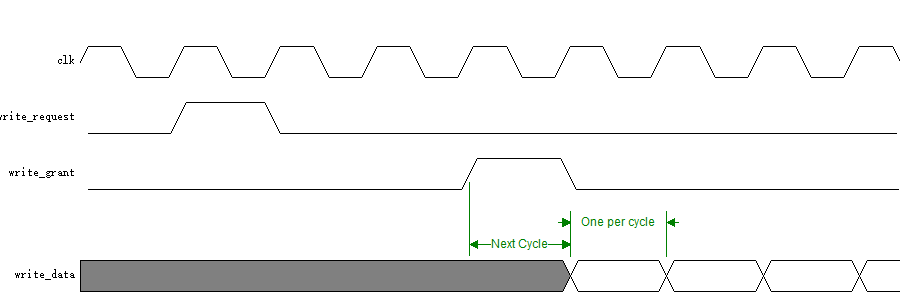
\includegraphics[width=\textwidth]{images/timing.png}
\end{figure}

Let's take a simple bus interface as an example. An accelerator can initiate a burst write of an arbitrary length, it first sends a request to the bus arbiter and waits for the grant. The grant can come any time after the request. But right after the grant the accelerator should sends the data on the data port one per cycle. So there is timing requirement between grant and data write. The timing diagram is shown in Figure \ref{fig:timing}. An example template of the write interface is shown below. The key idea in modeling timing charateristic is to use a counter to count the cycle. And when writing the refinement relations, define the matching between the behavior of the implementation in each cycle with each step in the sub-instructions in ILA.


\lstinputlisting{code/timingExample.py}



